\subsubsection{TAXII}

El objetivo que plantea Trusted Automated eXchange of Indicator Information (TAXII) es extender la capacidad de compartir indicadores, 
siendo dichos intercambios robustos, seguros y de gran volumen de datos. A su 
vez, los datos intercambiados deberían ser mas expresivos que en la actualidad.

Con TAXII no se busca crear una comunidad para compartir, sino que se le da a 
las organizaciones una herramienta que facilite el intercambio entre ellas. 
TAXII mejora las deficiencias existentes dando especificaciones abiertas y 
comunes para transportar los mensajes con información. También se provee un 
conjunto de capacidades como encriptación, autenticación, direccionamiento, 
alertas y pedidos entre sistemas.

TAXII es un conjunto de especificaciones técnicas y de documentación para 
permitir el intercambio de información procesable entre organizaciones. Para 
realizar dichos intercambios, se definen protocolos y formatos de datos que 
permiten intercambiar información de forma segura. Ha sido diseñado para permitir la
interoperabilidad de diferentes soluciones en lugar de ligarse a una tecnología o producto en particular.
Además, se busca incentivar a los proveedores de tecnología a incorporar soporte para las especificaciones
de TAXII en sus productos. La información intercambiada 
ayuda a detectar, prevenir y mitigar amenazas informáticas en tiempo real. Es 
importante recalcar que no se buscan definir acuerdos para el intercambio de 
información o gobierno. En su lugar, permite a las organizaciones mejorar el 
contexto en el que se encuentran respecto a las nuevas amenazas y además 
compartir la información que ellos elijan con las organizaciones que deseen de 
forma simple y rápida aprovechando las relaciones y sistemas existentes.

En el desarrollo de TAXII se buscó consenso y participación de la comunidad. 
TAXII permite el intercambio de información sobre amenazas de forma eficiente y 
comprensiva por medio de \emph{automatización} y \emph{articulación} de un 
modelo detallado de información. Para lograr esto, se utiliza una representación 
estándar de información de amenazas y un framework para soportar el intercambio 
de datos. El modelo permite el envío y recepción de un conjunto amplio de 
información de seguridad para soportar las necesidades referentes al intercambio 
de información. Se le da la libertad a los proveedores de determinar como sus 
productos producen, consumen o toman ventaja de los flujos de información 
especificados por TAXII.

 
\begin{figure}[ht!]
  \centering
    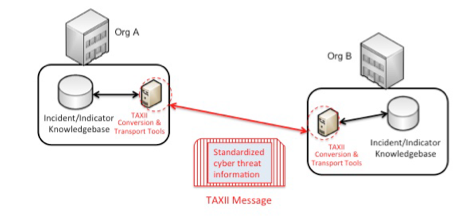
\includegraphics[width=150mm]{./images/TAXIIArchitecture1.png}
    \caption{Arquitectura de TAXII \protect\cite{b1}}
\end{figure}


TAXII cubre un amplio número de casos de uso, tecnologías, especificaciones e 
implementaciones. Los casos de uso son desarrollados de manera secuencial, 
permitiendo un conjunto inicial de casos de usos que permiten el intercambio de 
información. TAXII utiliza protocolos y especificaciones existentes siempre que 
es posible, de esta forma se integra con mecanismos de intercambio de 
información para reducir los costos de implementación y permitir la adopción 
rápida por parte de organizaciones ya establecidas y que se encuentran 
intercambiando información.

Las motivaciones para tener una mejor solución que permita intercambiar 
información lleva a que en el diseño de TAXII se hayan planteado los siguientes 
objetivos:
 \begin{itemize}
   \item Permitir el intercambio seguro y rápido de información referente a 
   amenazas entre comunidades de defensores de seguridad.
   \item Lograr un estándar para permitir compartir indicadores entre otros 
   elementos entre organizaciones.
   \item Extender el intercambio de indicadores para permitir intercambios 
   seguros, robustos y de gran volumen que tengan una expresividad mayor a la 
   actual.
   \item Soportar un amplio número de casos de uso y practicas comunes a las 
   comunidades.
   \item Tomar los estándares existentes que sean adecuados.
   \item Llegar a una adopción por parte de organizaciones internacionales de 
   estándares.
 \end{itemize}

Para representar la información, TAXII utiliza STIX. STIX es un 
lenguaje desarrollado por la comunidad para la especificación, captura, 
representación y comunicación de información de amenazas cibernéticas de forma 
estandarizada.

Para automatizar el intercambio de información, es necesario especificar como 
ésta es compartida. Para lograr esto, TAXII define especificaciones técnicas y 
documentación de soporte. En particular, las especificaciones de TAXII definen 
un conjunto de capacidades necesarias para el transporte exitoso de mensajes. 
Los mensajes TAXII llevan datos de amenazas informáticas transformadas a 
formato STIX. El conjunto completo de los mensajes incluyen mensajes con datos y 
de control.

TAXII utiliza protocolos y especificaciones existentes siempre que sea posible y 
los integra con los mecanismos actuales para reducir los costos de 
implementación y permitir una adopción rápida por parte de las organizaciones ya 
establecidas y que ya comparten información. TAXII ha sido desarrollado de forma 
modular para soportar una variedad de mecanismos y formatos de datos para ser 
intercambiados.

\paragraph{Casos de uso}

TAXII ha sido desarrollado para soportar casos de uso comunes para el 
intercambio de información. A continuación se detallan los casos de uso 
desarrollados.

\subparagraph{Alertas o Advertencias públicas}

Estas son advertencias al público en general o a varios miembros de CSIRTs, son 
enviadas a todos los subscriptores. Estas alertas son de una naturaleza muy 
amplia, por ello no necesitan ser encriptadas o tener autorizaciones especiales. 
Sin embargo es importante asegurar la autenticidad del emisor. Las entidades u 
organizaciones deben ser especificadas para identificar la fuente de la alerta.

\subparagraph{Alertas y reportes privados}

Las alertas privadas son similares a las públicas, la diferencia radica en que 
la información compartida es sensible y restringida a los socios que 
comparten datos. Los mecanismos para enviar datos deberían ser similares a los 
de las alertas públicas. Como las alertas y reportes se suponen sensibles y no 
para el uso general, es importante que TAXII soporte formas adecuadas de 
encriptación, autenticación, autorización e identificación de datos. Dependiendo 
en la naturaleza de las comunicaciones, podría requerirse un manejo explícito de 
marcas o restricciones.

Las alertas son generalmente cortas, teniendo mensajes estándar con indicadores 
muy específicos o acciones especificadas. Los reportes tienden a ser mas largos 
y pueden incluir reportes de incidentes, análisis de malware o amenazas así como 
otras observaciones.

\subparagraph{Soporte para Consultas}

Es común que los analistas busquen información entre sus comunidades así como 
por fuera de ellas. Para esto se soportan dos tipos de mensajes:
\begin{itemize}
  \item Request For Information (RFI): es un mensaje simple que se espera sea 
  manejado de forma manual y que permite que se pida información a otra 
  organización.
  \item Repository Search: Para este tipo de consulta, es esperado que una 
  organización ofrezca repositorios en los cuales buscar, los cuales podrían ser 
  compatibles con TAXII o STIX.
\end{itemize}

\subparagraph{Transferencia}

Varias organizaciones que transfieren información necesitan en algunas 
instancias agregar miembros. El nuevo miembro necesita obtener los datos del 
repositorio de alguna organización. Por ello se desea un caso de uso para 
realizar un intercambio de un gran volumen de datos.

\paragraph{Componentes de TAXII}

Como se dijo anteriormente, TAXII es un conjunto de especificaciones técnicas y 
documentación para el intercambio de información. A continuación se enumeran los 
distintos componentes de TAXII.

\begin{itemize}
  \item Especificación de TAXII: Define la especificación de los componentes y 
  provee una guía y requerimientos sobre como dichas especificaciones 
  interactúan en TAXII.
  \item Especificación de servicios TAXII: Define una serie de servicios que 
  deben ser implementados para ser compatible con TAXII. Describe la información 
  intercambiada en alto nivel y no se limita  ningún mecanismo de intercambio en 
  especial.
  \item Implementación de servicios: Se realiza una implementación de los 
  servicios TAXII para un mecanismo de intercambio. Cada implementación de 
  servicios provee una guía técnica y requerimientos para implementar la 
  especificación de los mecanismos de intercambio.
  \item Modelo de datos de mensajes: Se define una estructura para los mensajes 
  TAXII, incluyendo cabezales, datos del mensaje, control y mensajes de datos. 
  Los mensajes de datos utilizan STIX como carga de los mensajes TAXII.
  \item Implementación de los mensajes de datos: Es una implementación del 
  modelo de datos de mensajes, incluyendo la carga STIX. Cada implementación de 
  mensajes define una guía técnica y requerimientos para utilizar un formato de 
  mensajes particular para expresar el modelo de datos de mensaje.
\end{itemize}

\subparagraph{TAXII Toolkit}

Es provisto para soportar la adopción de TAXII y asistir en el desarrollo de 
capacidades compatibles. El toolkit provee una colección de implementaciones de 
referencia, un conjunto de herramientas y una colección de librerías e 
interfaces.

TAXII está definido por múltiples especificaciones relacionadas. Esta sección 
describe las especificaciones definidas en TAXII.

\begin{itemize}
  \item Especificación de servicios: Provee los requerimientos por los cuales se 
  definen los servicios e intercambios de TAXII. No provee detalles respecto al 
  formato de los datos o como los mensajes TAXII son transportados por la red. 
  Dichos detalles y requerimientos pueden ser encontrados en la especificación 
  de los protocolos de enlace y en la especificación de mensajes de enlace.
 \item Especificación de protocolos de enlace: Define los requerimientos para 
 transportar mensajes TAXII por la red. Puede haber varias especificaciones 
 creadas para TAXII. Cada especificación define requerimientos para el 
 transporte de mensajes TAXII utilizando protocolos de red y se proveen 
 requerimientos respecto a como los servicios TAXII son soportados por los 
 protocolos de red.
 \item Especificación de mensajes de enlace: Se definen requerimientos para 
 representar mensajes TAXII en un formato particular. Puede haber múltiples 
 especificaciones para dichos mensajes. Se provee información detallada sobre 
 como las especificaciones definidas en la especificación de servicios son 
 expresadas en los mensajes.
\end{itemize}

\begin{figure}[ht!]
  \centering
    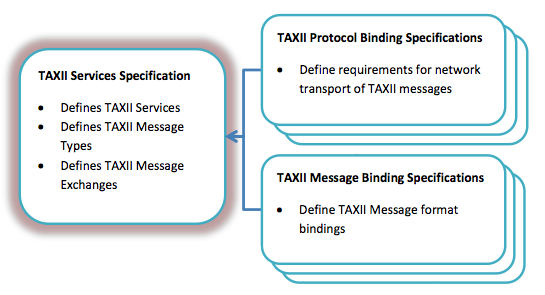
\includegraphics[width=150mm]{./images/TAXIIEspecification.png}
    \caption{Relación de las especificaciones de TAXII \protect\cite{b1}}
\end{figure}

Para dar flexibilidad en el proceso evolutivo de TAXII, se han separado las 
especificaciones de servicios, de los protocolos de enlace y de los mensajes de 
enlace. Lo dicho anteriormente es expresado en la figura 3.
Debido a que las organizaciones generalmente tienen restricciones 
respecto a los protocolos que soportan, TAXII busca no ligarse a un único 
protocolo que excluya a una parte de la comunidad. Cuando se ve que la comunidad 
expresa interés en un nuevo protocolo o tipo de mensaje, TAXII puede dar soporte 
para ellos sin cambiar los componentes centrales.

Dos grupos que usen el mismo protocolo de red y formato de mensajes serán 
capaces de intercambios de información estructurada de forma automática. Las 
políticas de intercambio de los participantes pueden limitar estos intercambios 
si es necesario, pero el uso de servicios compatibles con TAXII asegura que se 
puede intercambiar cualquier información con los mecanismos definidos por TAXII. 
Los grupos que usen diferentes protocolos o formatos de mensajes no serán 
capaces de comunicarse directamente, pero como están utilizando mensajes y 
servicios en el núcleo de las comunicaciones de sus comunidades significa que es 
posible establecer caminos para que ocurra la interacción.

\subparagraph{Especificación de Servicios}

Esta especificación provee normativas respecto a los servicios, mensajes e 
intercambios de mensajes en TAXII. No provee detalles respecto a como los 
mensajes son transportados, dejando eso a la especificación de los protocolos de 
enlace. Se da información respecto a los datos presentes en los mensajes TAXII y 
no a como los mensajes son expresados.

Las unidades funcionales de TAXII representan conjuntos discretos de actividades 
requeridas para soportar TAXII. Una unidad funcional representa algún componente 
con un rol bien definido en TAXII.

\begin{itemize}
  \item TAXII Transfer Agent (TTA): Es una unidad funcional conectada a la red 
  que envía o recibe mensajes TAXII. Una TTA interactúa con otras TTAs por medio 
  de la red y maneja los requerimientos de una o más de las especificaciones de 
  los protocolos de enlace. Una TTA provee un mensaje TAXII a un TAXII Message 
  Handler permitiendo que éste último sea independiente del protocolo de red 
  utilizado. De la misma forma, el TTA puede ser independiente del contenido de 
  los mensajes TAXII, dejando el manejo de la información al TAXII Message 
  Handler.
  \item TAXII Messsage Handler (TMH): Es una unidad funcional que produce y 
  consume mensajes TAXII. EL TMH es responsable de parsear y construir mensajes 
  con el formato especificado en uno o más TAXII Message Binding Specifications. 
  Un TMH interactúa con un TTA, el cual maneja los detalles necesarios para 
  transmitir mensajes por la red. El Backend TAXII interactúa con el TMH para 
  convertir su contenido en mensajes TAXII y llevar a cabo actividades basadas 
  en los mensajes TAXII que son recibidos por el TMH.
  \item TAXII Backend: Cubre todas las unidades funcionales distintas al TTA y 
  al TMH. Las especificaciones de TAXII no proveen requerimientos sobre como son 
  implementadas las capacidades en un backend más allá de como debe interactuar 
  con el TMH. Las organizaciones o implementadores pueden decidir que 
  capacidades implementar según los servicios TAXII que deseen soportar o según 
  como quieran dar ese soporte.
  \item Arquitectura TAXII: Cubre los aspectos de las unidades funcionales de la 
  infraestructura de productor o consumidor que provee o utiliza servicios 
  TAXII. Una arquitectura TAXII incluye una TTA, un TMH y un backend TAXII.
  \end{itemize}

\begin{figure}[ht!]
  \centering
    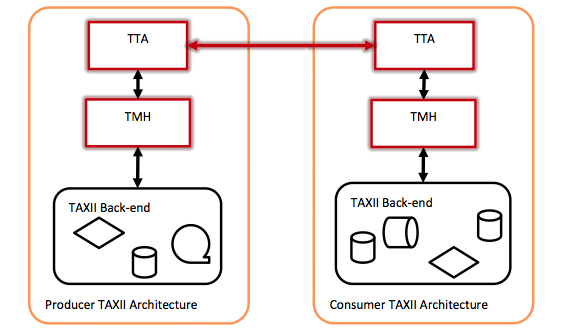
\includegraphics[width=150mm]{./images/TAXIIArchitecture.png}
    \caption{Unidades funcionales de TAXII \protect\cite{b1}}
\end{figure}

\paragraph{Capacidades}

TAXII provee capacidades especificas para aquellos que desean compartir 
información de amenazas cibernéticas. Las capacidades TAXII son el nivel más 
alto en el cual se pueden expresar las acciones de TAXII. Hay tres capacidades 
que soporta la actual versión de TAXII, estas son: push messaging, pull 
messaging y discovery.

En push messaging la información puede ser enviada de un productor a un 
consumidor. Esto puede reflejar una relación pre-existente entre el productor y 
el consumidor en la que el consumidor ha pedido que se le envíen datos desde el 
productor. También puede usarse en caso de que el consumidor desee aceptar 
contribuciones de cualquier productor, y estos le envíen datos en cualquier 
momento.

Pull messaging permite a un consumidor requerir información de un productor. 
Esto no solo le permite al consumidor el control sobre el momento en el que 
recibe los datos sino que también le permite hacerlo sin tener que aceptar 
conexiones entrantes. Así como en push messaging, el productor y consumidor 
pueden tener acuerdos pre-existentes para que el consumidor tenga acceso a los 
datos del productor. De forma alternativa, un productor puede hacer su 
información pública de forma que cualquier consumidor pueda obtenerla. La 
versión actual de pull messaging limita a los consumidores a hacer pedidos por 
medio de las organizaciones productoras de los datos en lugar de por los datos 
en si. Toda la información provista por un productor debe estar organizada en 
grupos llamados "TAXII Data Feeds". Cada elemento en un TAXII data feed es 
etiquetado utilizando timestamps. El productor tiene total dominio sobre como el 
contenido se mapea en TAXII data feeds y en el significado de los timestamps. La 
capacidad de pull messaging está atada a entender el contenido del productor.

Para facilitar las comunicaciones automatizadas, TAXII soporta capacidades para 
descubrir los servicios específicos que ofrece un servidor o grupo de 
servidores, así como los protocolos o mensajes que este servidor ofrece. Esto no 
quita la necesidad de que personas estén involucradas para establecer acuerdos de 
cooperación lo cual esta por fuera del objetivo de TAXII. Sin embargo, permite 
el intercambio de información respecto a las capacidades que un productor 
soporta y cuales son los mecanismos que utiliza para hacerlo.

\paragraph{Servicios TAXII}

Los servicios TAXII representan un conjunto de mecanismos necesarios para 
soportar capacidades TAXII. Una implementación TAXII pudiera implementar alguno, 
todos o incluso ninguno de los servicios definidos.
TAXII define los siguientes servicios:
\begin{itemize}
  \item Servicio de descubrimiento: Es utilizado para recibir y responder a 
  mensajes que requieren información sobre los servicios ofrecidos.
  \item Feed Managment Service: Es utilizado para recibir o responder a mensajes 
  utilizados para el manejo de subscripciones a TAXII Data Feed.
  \item Inbox Service: Es utilizado para recibir información de amenazas 
  cibernéticas por medio de intercambios iniciados por el productor en intervalos 
  dictados por este.
  \item Poll Service: Es utilizado para recibir y responder a mensajes de pedido 
  a el TAXII Data Feed iniciados por el consumidor.
\end{itemize}

A continuación se describen los distintos servicios.

\subparagraph{Discovery Service}

Es un mecanismo para comunicar información referente al uso de servicios TAXII y 
a su disponibilidad. Para un pedido al servicio, se retorna una lista de los 
servicios TAXII y como estos pueden ser invocados. Un solo servicio de 
descubrimiento puede reportar servicios TAXII en diferentes equipos finales o 
incluso en múltiples organizaciones, los propietarios del servicio pueden 
definir su alcance a gusto. Un servicio de descubrimiento puede utilizar 
varios factores para determinar cuales servicios revelar ante una petición, 
incluyendo, pero no limitado a la entidad del cliente TAXII.
El servicio de descubrimiento debe soportar "Discovery Message Exchange".

\subparagraph{Feed Managment Service}

Es el mecanismo con el cual un consumidor pide información referente a TAXII 
Data Feeds, pidiendo subscripciones a estos, o modificando las existentes. Este 
servicio facilita el intercambio de mensajes para manejar las subscripciones. 
No se entrega contenido de los TAXII Data Feed, en su lugar se envía 
contenido del TAXII Data Feed al servicio de Inbox de un consumidor en intercambios 
iniciados por un productor o en respuesta directa a un pedido del consumidor al 
servicio de poll.
Dicho servicio debe implementar soporte para subscription managment exchange.
Dicho servicio podría implementar soporte de feed information exchange.

\subparagraph{Inbox service}
Este servicio es el mecanismo con el cual un consumidor acepta los mensajes en 
un intercambio iniciado por el productor. Un consumidor puede implementarlo 
para recibir datos del TAXII Data Feed.
El servicio de inbox debe implementar soporte para Data Push Exchange.

\subparagraph{Poll service}
Es provisto por un productor para permitir pedidos al TAXII Data Feed iniciados 
por  el consumidor. Un consumidor contacta a este servicio explícitamente 
pidiendo el contenido del TAXII Data Feed. Los productores podrían ofrecer Data 
Feeds combinando envíos al Inbox service del consumidor o por medio de pedidos 
al servicio de poll de productor.
Una implementación de éste servicio debe dar soporte a Data Poll Exchange.

\paragraph{Intercambio de mensajes TAXII}

Esta sección describe los mensajes intercambiados que son necesarios para soportar 
los servicios definidos antes. Estos intercambios solo consideran mensajes 
TAXII y son independientes a los protocolos sobre los cuales viajan los mensajes.
 En particular, esos protocolos podrían requerir intercambios de red 
adicionales antes de transmitir mensajes TAXII o romper un mensaje TAXII en 
múltiples mensajes del protocolo subyacente que son transmitidos 
independientemente. Los siguientes diagramas representan conceptualmente la 
secuencia en la cual los mensajes TAXII son transmitidos y como actúan.

\subparagraph{Data Push Exchange}
En este intercambio, un mensaje STIX es transmitido desde un cliente a un 
servidor inbox que está esperando. El mensaje STIX puede ser solicitado o no 
solicitado. El servidor inbox puede ser capaz de filtrar mensajes según la 
autenticidad del emisor. Los mensajes enviados en este intercambio no deberían 
tener un campo 'In Response to' en su header.

\begin{figure}[ht!]
  \centering
    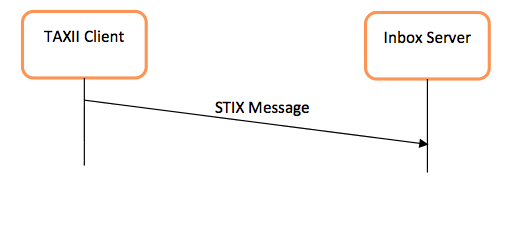
\includegraphics[width=150mm]{./images/DataPushExchange.png}
    \caption{Mensajes intercambiados en un Data Push Exchange \protect\cite{b1}}
\end{figure}

El cliente TAXII envía un mensaje STIX al inbox server. El inbox server podría 
descartar el mensaje o pasar el mensaje STIX junto con cualquier información de 
la entidad autenticada al Back-end TAXII. El cliente TAXII no recibe respuesta 
del servidor de inbox y no sabrá si el mensaje ha sido aceptado o descartado por 
el servidor, aunque el protocolo confiable de la capa inferior puede asegurar 
que el mensaje fue entregado a la TTA del servidor de inbox. El inbox server no 
enviará un mensaje de error TAXII si hay algún problema con el mensaje TAXII.

\subparagraph{Discovery Exchange}

Un cliente TAXII pide información sobre el servicio TAXII ofrecido por un 
productor. El discovery server del productor responde con una lista de 
servicios. Si bien el cliente puede ser informado de la existencia de un 
servicio, este no necesariamente tendrá acceso inmediato al servicio.

\begin{figure}[ht!]
  \centering
    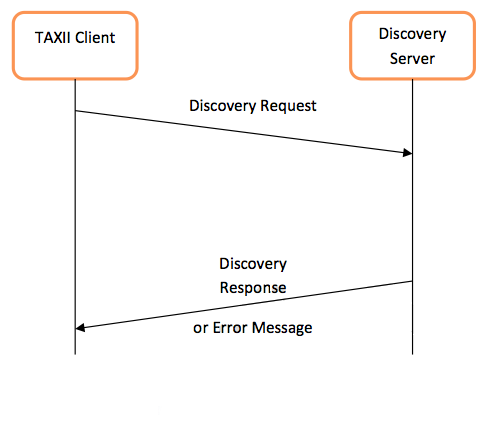
\includegraphics[width=150mm]{./images/DiscoveryExchange.png}
     \caption{Mensajes intercambiados en un Discovery Exchange \protect\cite{b1}}
\end{figure}

El cliente TAXII envía un pedido de descubrimiento al servidor. Cuando el 
servidor recibe el pedido puede retornar un mensaje de error o pasar la 
información al Backend TAXII. Información relevante incluye la identidad 
autenticada si ésta fue provista. El Backend TAXII podría utilizar esta 
información junto a su propia política de control de acceso  para crear una 
lista de servicios a ser retornada. Esto podría ser empaquetado en una 
respuesta de discovery lo cuales podrían ser enviados al cliente TAXII. El 
cliente TAXII recibe esa respuesta y la pasa la información del servicio a su 
propio Back-End para ser procesado.

\subsection{Feed Information Exchange}

En éste intercambio un cliente TAXII pide información sobre fuentes de datos disponibles en 
un Feed Server. El servidor responde con una lista de fuentes de datos 
disponibles. Dicha respuesta es realizada por el backend y en ella se pueden considerar 
decisiones de control de acceso para realizar la respuesta.

\begin{figure}[ht!]
  \centering
    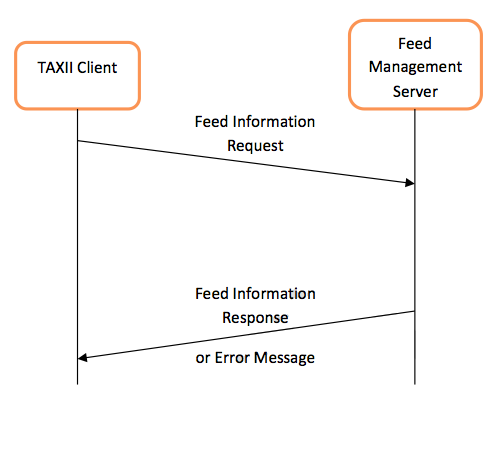
\includegraphics[width=150mm]{./images/FeedInformationExchange.png}
    \caption{Mensajes intercambiados en un Feed Information Exchange \protect\cite{b1}}
\end{figure}

El cliente TAXII envía el Feed Information Request al 
servidor. Cuando el servidor recibe la request podría retornar un mensaje de 
error o pasar la información relevante al TAXII backend. Entre la información 
relevante se podría incluir la identidad. El backend podría utilizar esta 
información junto con sus políticas de control de acceso para crear una lista de 
fuentes de datos para ser enviadas al cliente. Esta lista es empaquetada en una 
Feed Information Response. El cliente recibe este mensaje y pasa el Feed a su 
propio backend para ser procesado.

\subsection{Subscription Managment Exchange}

En este un cliente intenta establecer, borrar, pausar, resumir o modificar una 
subscripción a un TAXII Data Feed conocido enviando un mensaje subscription 
managment request al servidor. El servidor pasa la request al TAXII Back-end el 
cual determina la respuesta. Esta respuesta es luego enviada al cliente.

\begin{figure}[ht!]
  \centering
    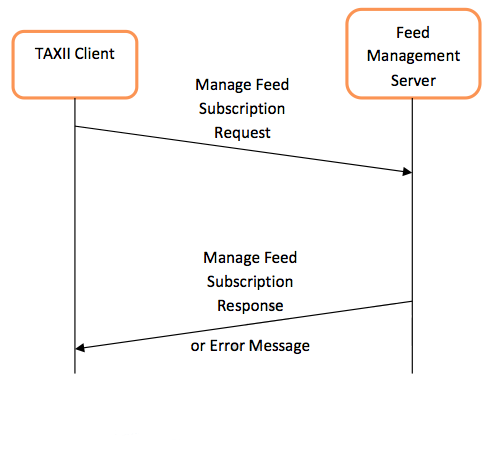
\includegraphics[width=150mm]{./images/SubscriptionManagmentExchange.png}
    \caption{Mensajes intercambiados en un Subscription Managment Exchange \protect\cite{b1}} 
\end{figure}

El cliente TAXII envía una Manage Feed Subscription Request al servidor. Éste 
podría retornar un mensaje de error TAXII o pasar la información relevante al 
TAXII backend. La información relevante podría incluir la identidad, parámetros 
que identifiquen la subscripción a ser modificada o creada, y la acción 
realizada. El backend TAXII puede usar dicha información junto con sus 
políticas de control de acceso y las funcionalidades que posea para determinar 
si la acción está permitida o no. Dependiendo de la respuesta, el servidor 
podría retornar un mensaje de error TAXII o enviar una respuesta Manage Feed 
Successful Response.

\subsection{Feed Poll Exchange}

Es utilizado por un consumidor para pedir contenido de un productor de datos. El 
TAXII Data Feed content es enviado al consumidor en el mismo intercambio. Esto  
permite a un consumidor devolver el Data Feed Content en su propia tabla de 
tiempo y sin necesidad de utilizar un Inbox Server o aceptar conexiones 
entrantes.

\begin{figure}[ht!]
  \centering
    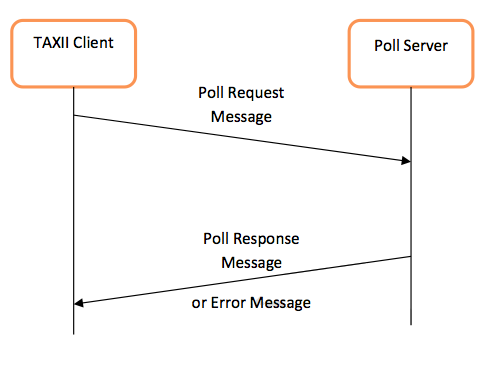
\includegraphics[width=150mm]{./images/FeedPollExchange.png}
    \caption{Mensajes intercambiados en un Feed Poll Exchange \protect\cite{b1}}
\end{figure}

El cliente consumidor inicia el intercambio enviando un mensaje Poll Request al 
servidor de Poll del productor. El servidor puede enviar un mensaje de error 
inmediatamente o pasar la información relevante al TAXII backend. Información 
relevante incluye el nombre de la fuente, los parámetros de subscripción, 
timestamps indicando el intervalo de tiempo de la información que pide el 
consumidor y la identidad del consumidor. El backend TAXII evalúa ésta
información para determinar la respuesta. Las respuesta posibles:
\begin{itemize}
  \item El pedido de información podría ser denegado. En este caso el servidor 
  de poll crea un error TAXII 
  \item Un conjunto de contenido TAXII Data Feed podría ser provisto. En este 
  caso, el servidor de Poll construirá y enviará un mensaje de Poll Response. 
  Este mensaje indica el intervalo de tiempo que cubre el TAXII Data Feed que es 
  transmitido y los cuerpos de mensajes STIX que forman el contenido del TAXII 
  Data Feed.
\end{itemize}
En todos los casos, el cliente TAXII recibe el mensaje apropiado y pasa esta 
información al Backend TAXII para ser procesado.

